\chapter{Application to Arrhythmia Detection}

% use Times
%\usepackage{times}
% For figures
%\usepackage{graphicx} % more modern

% For Tables
%\usepackage{booktabs}      % professional-quality tables

% For citations
%\usepackage{natbib}

% For algorithms
%\usepackage{algorithm}
%\usepackage{algorithmic}
%\usepackage[caption = false]{subfig}
%\usepackage{hyperref}
%\usepackage{array}

% Packages hyperref and algorithmic misbehave sometimes.  We can fix
% this with the following command.
%\newcommand{\theHalgorithm}{\arabic{algorithm}}

% TODO figure out labelling
\section{Introduction}
\label{sec:arrhythmias:intro}

We develop a model which can diagnose irregular heart rhythms, also known as
arrhythmias, from single-lead ECG signals better than a cardiologist. Key to
exceeding expert performance is a deep convolutional network which can map a
sequence of ECG samples to a sequence of arrhythmia annotations along with a
novel dataset two orders of magnitude larger than previous datasets of its
kind.

Many heart diseases, including Myocardial Infarction, AV Block, Ventricular
Tachycardia and Atrial Fibrillation can all be diagnosed from ECG signals with
an estimated 300 million ECGs recorded annually~\cite{heden1996detection}. We
investigate the task of arrhythmia detection from the ECG record. This is known
to be a challenging task for computers but can usually be determined by an
expert from a single, well-placed lead.

Arrhythmia detection from ECG recordings is usually performed by expert
technicians and cardiologists given the high error rates of computerized
interpretation.  One study found that of all the computer predictions for
non-sinus rhythms, only about 50\% were correct~\cite{shah2007errors}; in
another study, only 1 out of every 7 presentations of second degree AV block
were correctly recognized by the algorithm~\cite{guglin2006common}. To
automatically detect heart arrhythmias in an ECG, an algorithm must implicitly
recognize the distinct wave types and discern the complex relationships between
them over time. This is difficult due to the variability in wave morphology
between patients as well as the presence of noise.

We train a 34-layer convolutional neural network (CNN) to detect arrhythmias in
arbitrary length ECG time-series. Figure~\ref{fig:record} shows an example of
an input to the model. In addition to classifying noise and the sinus rhythm,
the network learns to classify and segment twelve arrhythmia types present in
the time-series. The model is trained end-to-end on a single-lead ECG signal
sampled at 200Hz and a sequence of annotations for every second of the ECG as
supervision. To make the optimization of such a deep model tractable, we use
residual connections and batch-normalization~\cite{he2016deep, ioffe2015batch}.
The depth increases both the non-linearity of the computation as well as the
size of the context window for each classification decision.

We construct a dataset 500 times larger than other datasets of its
kind~\cite{moody2001impact, goldberger2000physiobank}. One of the most popular
previous datasets, the MIT-BIH corpus contains ECG recordings from 47 unique
patients. In contrast, we collect and annotate a dataset of about 30,000 unique
patients from a pool of nearly 300,000 patients who have used the Zio Patch
monitor\footnote[1]{iRhythm Technologies, San Francisco,
California}~\cite{turakhia2013diagnostic}. We intentionally select patients
exhibiting abnormal rhythms in order to make the class balance of the dataset
more even and thus the likelihood of observing unusual heart-activity high.

We test our model against board-certified cardiologists. A committee of three
cardiologists serve as gold-standard annotators for the 336 examples in the
test set. Our model exceeds the individual expert performance on both recall
(sensitivity), and precision (positive predictive value) on this test set.

\section{Related Work}
\label{sec:arrhythmia:related}

Automatic high-accuracy methods for R-peak extraction have existed at least
since the mid 1980's \cite{pan1985real}. Current algorithms for R-peak
extraction tend to use wavelet transformations to compute features from the raw
ECG followed by finely-tuned threshold based classifiers \cite{li1995detection,
martinez2004wavelet}. Because accurate estimates of heart rate and heart rate
variability can be extracted from R-peak features, feature-engineered
algorithms are often used for coarse-grained heart rhythm classification,
including detecting tachycardias (fast heart rate), bradycardias (slow heart
rate), and irregular rhythms. However, such features alone are not sufficient
to distinguish between most heart arrhythmias since features based on the
atrial activity of the heart as well as other features pertaining to the QRS
morphology are needed.

Much work has been done to automate the extraction of other features from the
ECG. For example, beat classification is a common sub-problem of
heart-arrhythmia classification. Drawing inspiration from automatic speech
recognition, Hidden Markov models with Gaussian observation probability
distributions have been applied to the task of beat detection
\cite{coast1990approach}. Artificial neural networks have also been used for
the task of beat detection \cite{melo2000arrhythmia}. While these models have
achieved high-accuracy for some beat types, they are not yet sufficient for
high-accuracy heart arrhythmia classification and segmentation. For example,
\cite{artis1991detection} train a neural network to distinguish between Atrial
Fibrillation and Sinus Rhythm on the MIT-BIH dataset. While the network can
distinguish between these two classes with high-accuracy, it does not
generalize to noisier single-lead recordings or classify among the full range
of $15$ rhythms available in MIT-BIH. This is in part due to insufficient
training data, and because the model also discards critical information in the
feature extraction stage.

The most common dataset used to design and evaluate ECG algorithms is the
MIT-BIH arrhythmia database \cite{moody2001impact} which consists of 48
half-hour strips of ECG data. Other commonly used datasets include the MIT-BIH
Atrial Fibrillation dataset \cite{moody1983new} and the QT dataset
\cite{laguna1997database}. While useful benchmarks for R-peak extraction and
beat-level annotations, these datasets are too small for fine-grained
arrhythmia classification. The number of unique patients is in the single digit
hundreds or fewer for these benchmarks. A recently released dataset captured
from the AliveCor ECG monitor contains about 7000 records \cite{clifford2017}.
These records only have annotations for Atrial Fibrillation; all other
arrhythmias are grouped into a single bucket. The dataset we develop contains
29,163 unique patients and $14$ classes with hundreds of unique examples for
the rarest arrhythmias.

Machine learning models based on deep neural networks have consistently been
able to approach and often exceed human agreement rates when large annotated
datasets are available \cite{amodei2016deep, xiong2016achieving,he2015delving}.
These approaches have also proven to be effective in healthcare applications,
particularly in medical imaging where pretrained ImageNet models can be applied
\cite{esteva2017dermatologist, gulshan2016development}. We draw on work in
automatic speech recognition for processing time-series with deep convolutional
neural networks and recurrent neural networks \cite{hannun2014deepspeech,
sainath2013deep}, and techniques in deep learning to make the optimization of
these models tractable \cite{he2016deep, he2016identity, ioffe2015batch}.


%\begin{figure}[ht]
%  \centering
%  \includegraphics[width=\linewidth]{figs/main_figure.png}
%  \caption{
%    Our trained convolutional neural network correctly detecting the sinus rhythm (SINUS) and Atrial Fibrillation (AFIB) from this ECG recorded with a single-lead wearable heart monitor.
%  }
%  \label{fig:record}
%\end{figure}
%\section{Introduction}
\label{sec:scaling_asr:introduction}

Decades worth of hand-engineered domain knowledge has gone into current
state-of-the-art automatic speech recognition (ASR) pipelines.  A simple but
powerful alternative solution is to train such ASR models end-to-end, using
deep learning to replace most modules with a single
model~\cite{hannun2014deepspeech}. We present the second generation of our
speech system that exemplifies the major advantages of end-to-end learning. The
{Deep Speech 2} ASR pipeline approaches or exceeds the accuracy of Amazon
Mechanical Turk human workers on several benchmarks, works in multiple
languages with little modification, and is deployable in a production setting.
It thus represents a significant step towards a single ASR system that
addresses the entire range of speech recognition contexts handled by humans.
Since our system is built on end-to-end deep learning, we can employ a spectrum
of deep learning techniques: capturing large training sets, training larger
models with high performance computing, and methodically exploring the space of
neural network architectures. We show that through these techniques we are able
to reduce error rates of our previous end-to-end
system~\cite{hannun2014deepspeech} in English by up to 43\%, and can also
recognize Mandarin speech with high accuracy.

One of the challenges of speech recognition is the wide range of variability in
speech and acoustics. As a result, modern ASR pipelines are made up of numerous
components including complex feature extraction, acoustic models, language and
pronunciation models, speaker adaptation, etc. Building and tuning these
individual components makes developing a new speech recognizer very hard,
especially for a new language.  Indeed, many parts do not generalize well
across environments or languages and it is often necessary to support multiple
application-specific systems in order to provide acceptable accuracy. This
state of affairs is different from human speech recognition: people have the
innate ability to learn any language during childhood, using general skills to
learn language. After learning to read and write, most humans can transcribe
speech with robustness to variation in environment, speaker accent and noise,
without additional training for the transcription task.  To meet the
expectations of speech recognition users, we believe that a single engine must
learn to be similarly competent; able to handle most applications with only
minor modifications and able to learn new languages from scratch without
dramatic changes.  Our end-to-end system puts this goal within reach, allowing
us to approach or exceed the performance of human workers on several tests in
two very different languages: Mandarin and English.

Since {Deep Speech 2} (DS2) is an end-to-end deep learning system, we can
achieve performance gains by focusing on three crucial components:  the model
architecture, large labeled training datasets, and computational scale. This
approach has also yielded great advances in other application areas such as
computer vision and natural language.  This paper details our contribution to
these three areas for speech recognition, including an extensive investigation
of model architectures and the effect of data and model size on recognition
performance.  In particular, we describe numerous experiments with neural
networks trained with the Connectionist Temporal Classification (CTC) loss
function~\cite{graves2006} to predict speech transcriptions from audio.  We
consider networks composed of many layers of recurrent connections,
convolutional filters, and nonlinearities, as well as the impact of a specific
instance of Batch Normalization~\cite{ioffe2015batch} (BatchNorm) applied to
RNNs.  We not only find networks that produce much better predictions than
those in previous work~\cite{hannun2014deepspeech}, but also find instances of
recurrent models that can be deployed in a production setting with no
significant loss in accuracy.

Beyond the search for better model architecture, deep learning systems benefit
greatly from large quantities of training data.  We detail our data capturing
pipeline that has enabled us to create larger datasets than what is typically
used to train speech recognition systems.  Our English speech system is trained
on 11,940 hours of speech, while the Mandarin system is trained on 9,400 hours.
We use data synthesis to further augment the data during training.

Training on large quantities of data usually requires the use of larger models.
Indeed, our models have many more parameters than those used in our previous
system. Training a single model at these scales requires tens of
exaFLOPs\footnote{1 exaFLOP = $10^{18}$ FLoating-point OPerations.} that would
require 3-6 weeks to execute on a single GPU. This makes model exploration a
very time consuming exercise, so we have built a highly optimized training
system that uses 8 or 16 GPUs to train one model. In contrast to previous
large-scale training approaches that use parameter servers and asynchronous
updates~\cite{dean2012, chilimbi2014}, we use synchronous SGD, which is easier
to debug while testing new ideas, and also converges faster for the same degree
of data parallelism. To make the entire system efficient, we describe
optimizations for a single GPU as well as improvements to scalability for
multiple GPUs. We employ optimization techniques typically found in High
Performance Computing to improve scalability. These optimizations include a
fast implementation of the CTC loss function on the GPU, and a custom memory
allocator. We also use carefully integrated compute nodes and a custom
implementation of all-reduce to accelerate inter-GPU communication. Overall the
system sustains approximately 50 teraFLOP/second when training on 16 GPUs. This
amounts to 3 teraFLOP/second per GPU which is about 50\% of peak theoretical
performance. This scalability and efficiency cuts training times down to 3 to 5
days, allowing us to iterate more quickly on our models and datasets.

We benchmark our system on several publicly available test sets and compare the
results to our previous end-to-end system~\cite{hannun2014deepspeech}.  Our
goal is to eventually reach human-level performance not only on specific
benchmarks, where it is possible to improve through dataset-specific tuning,
but on a range of benchmarks that reflects a diverse set of scenarios. To that
end, we have also measured the performance of human workers on each benchmark
for comparison.  We find that our system outperforms humans in some
commonly-studied benchmarks and has significantly closed the gap in much harder
cases.  In addition to public benchmarks, we show the performance of our
Mandarin system on internal datasets that reflect real-world product scenarios.

Deep learning systems can be challenging to deploy at scale.  Large neural
networks are computationally expensive to evaluate for each user utterance, and
some network architectures are more easily deployed than others. Through model
exploration, we find high-accuracy, deployable network architectures, which we
detail here. We also employ a batching scheme suitable for GPU hardware called
Batch Dispatch that leads to an efficient, real-time implementation of our
Mandarin engine on production servers.  Our implementation achieves a 98th
percentile compute latency of 67 milliseconds, while the server is loaded with
10 simultaneous audio streams.

%
%\section{Model}
%\label{model}
%\begin{figure}[ht!]
%  \centering
%  \includegraphics[height=15cm]{figs/ecg-nnet.pdf}
%  \caption{The architecture of the network. The first and last layer are special-cased due to the pre-activation residual blocks. Overall, the network contains 33 layers of convolution followed by a fully-connected layer and a softmax.}
%  \label{fig:net}
%\end{figure}
%
%
%\section{RNN Training Setup}
\label{sec:deepspeech:model}

The core of our system is a recurrent neural network (RNN) trained to ingest
speech spectrograms and generate English text transcriptions. Let a single
utterance $X$ and label $Y$ be sampled from a training set $\mathcal{X} =
\{(X^{(1)},Y^{(1)}),(X^{(2)},Y^{(2)}),\ldots\}$. Each utterance, $x^{(i)}$, is
a time-series of length $T^{(i)}$ where every time-slice is a vector of audio
features, $X_t^{(i)}, t=1,\ldots,T^{(i)}$. We use spectrograms as our features,
so $x^{(i)}_{t,p}$ denotes the power of the $p$'th frequency bin in the audio
frame at time $t$. The goal of our RNN is to convert an input sequence $X$ into
a sequence of character probabilities for the transcription $Y$, with
$\hat{y_t} = p(c_t \mid x)$, where $c_t \in \{\textrm{a,b,c,}\ldots,\textrm{z},
\textit{space},\textit{apostrophe},\textit{blank}\}$.

Our RNN model is composed of 5 layers of hidden units.  For an input $x$, the
hidden units at layer $l$ are denoted $h^{(l)}$ with the convention that
$h^{(0)}$ is the input. The first three layers are not recurrent. For the first
layer, at each time $t$, the output depends on the spectrogram frame $x_t$
along with a context of $C$ frames on each side.\footnote{We typically use
$C\in \{5, 7, 9\}$ for our experiments.} The remaining non-recurrent layers
operate on independent data for each time step. Thus, for each time $t$, the
first 3 layers are computed by:
\begin{align*}
    h^{(l)}_t &= g(W^{(l)} h^{(l-1)}_t + b^{(l)})
\end{align*}
where $g(z) = \min\{\max\{0,z\}, 20\}$ is the clipped rectified-linear (ReLu)
activation function and $W^{(l)}, b^{(l)}$ are the weight matrix and bias
parameters for layer $l$.\footnote{The ReLu units are clipped in order to keep
the activations in the recurrent layer from exploding; in practice the units
rarely saturate at the upper bound.} The fourth layer is a bi-directional
recurrent layer~\cite{schuster1997bidirectional}. This layer includes two sets
of hidden units: a set with forward recurrence, $h^{(f)}$, and a set with
backward recurrence $h^{(b)}$:
\begin{align*}
    h^{(f)}_t &= g(W^{(4)} h^{(3)}_t + W_r^{(f)} h^{(f)}_{t-1} + b^{(4)}) \\
    h^{(b)}_t &= g(W^{(4)} h^{(3)}_t + W_r^{(b)} h^{(b)}_{t+1} + b^{(4)})
\end{align*}
Note that $h^{(f)}$ must be computed sequentially from $t=1$ to $t=T^{(i)}$ for
the $i$'th utterance, while the units $h^{(b)}$ must be computed sequentially
in reverse from $t=T^{(i)}$ to $t=1$.

The fifth (non-recurrent) layer takes both the forward and backward units as
inputs $h^{(5)}_t = g(W^{(5)} h^{(4)}_t + b^{(5)})$ where $h^{(4)}_t =
h^{(f)}_t + h^{(b)}_t$. The output layer is a standard softmax function that
yields the predicted character probabilities for each time slice $t$ and
character $k$ in the alphabet:
\begin{align*}
    h_{t,k}^{(6)} = \hat{y}_{t,k} \equiv p(c_t = k \mid x) =
        \frac{\exp(W_k^{(6)} h_t^{(5)}+b_k^{(6)})}{\sum_j \exp(W_j^{(6)} h_t^{(5)}+b_j^{(6)})}.
\end{align*}
Here $W_k^{(6)}$ and $b_k^{(6)}$ denote the $k$'th row of the weight matrix and
$k$'th bias, respectively.  

Once we have computed a prediction for $p(c_t \mid x)$, we compute the CTC
loss~\cite{graves2006} to measure the error in prediction. During training, we
can evaluate the gradient of the loss with respect to the network outputs. From
this point, computing the gradient with respect to all of the model parameters
is done via back-propagation through the rest of the network. We use Nesterov's
Accelerated gradient method for training~\cite{sutskever2013}.\footnote{We use
momentum of 0.99 and anneal the learning rate by a constant factor, chosen to
yield the fastest convergence, after each epoch through the data.}

\begin{figure}[th]
\centering
 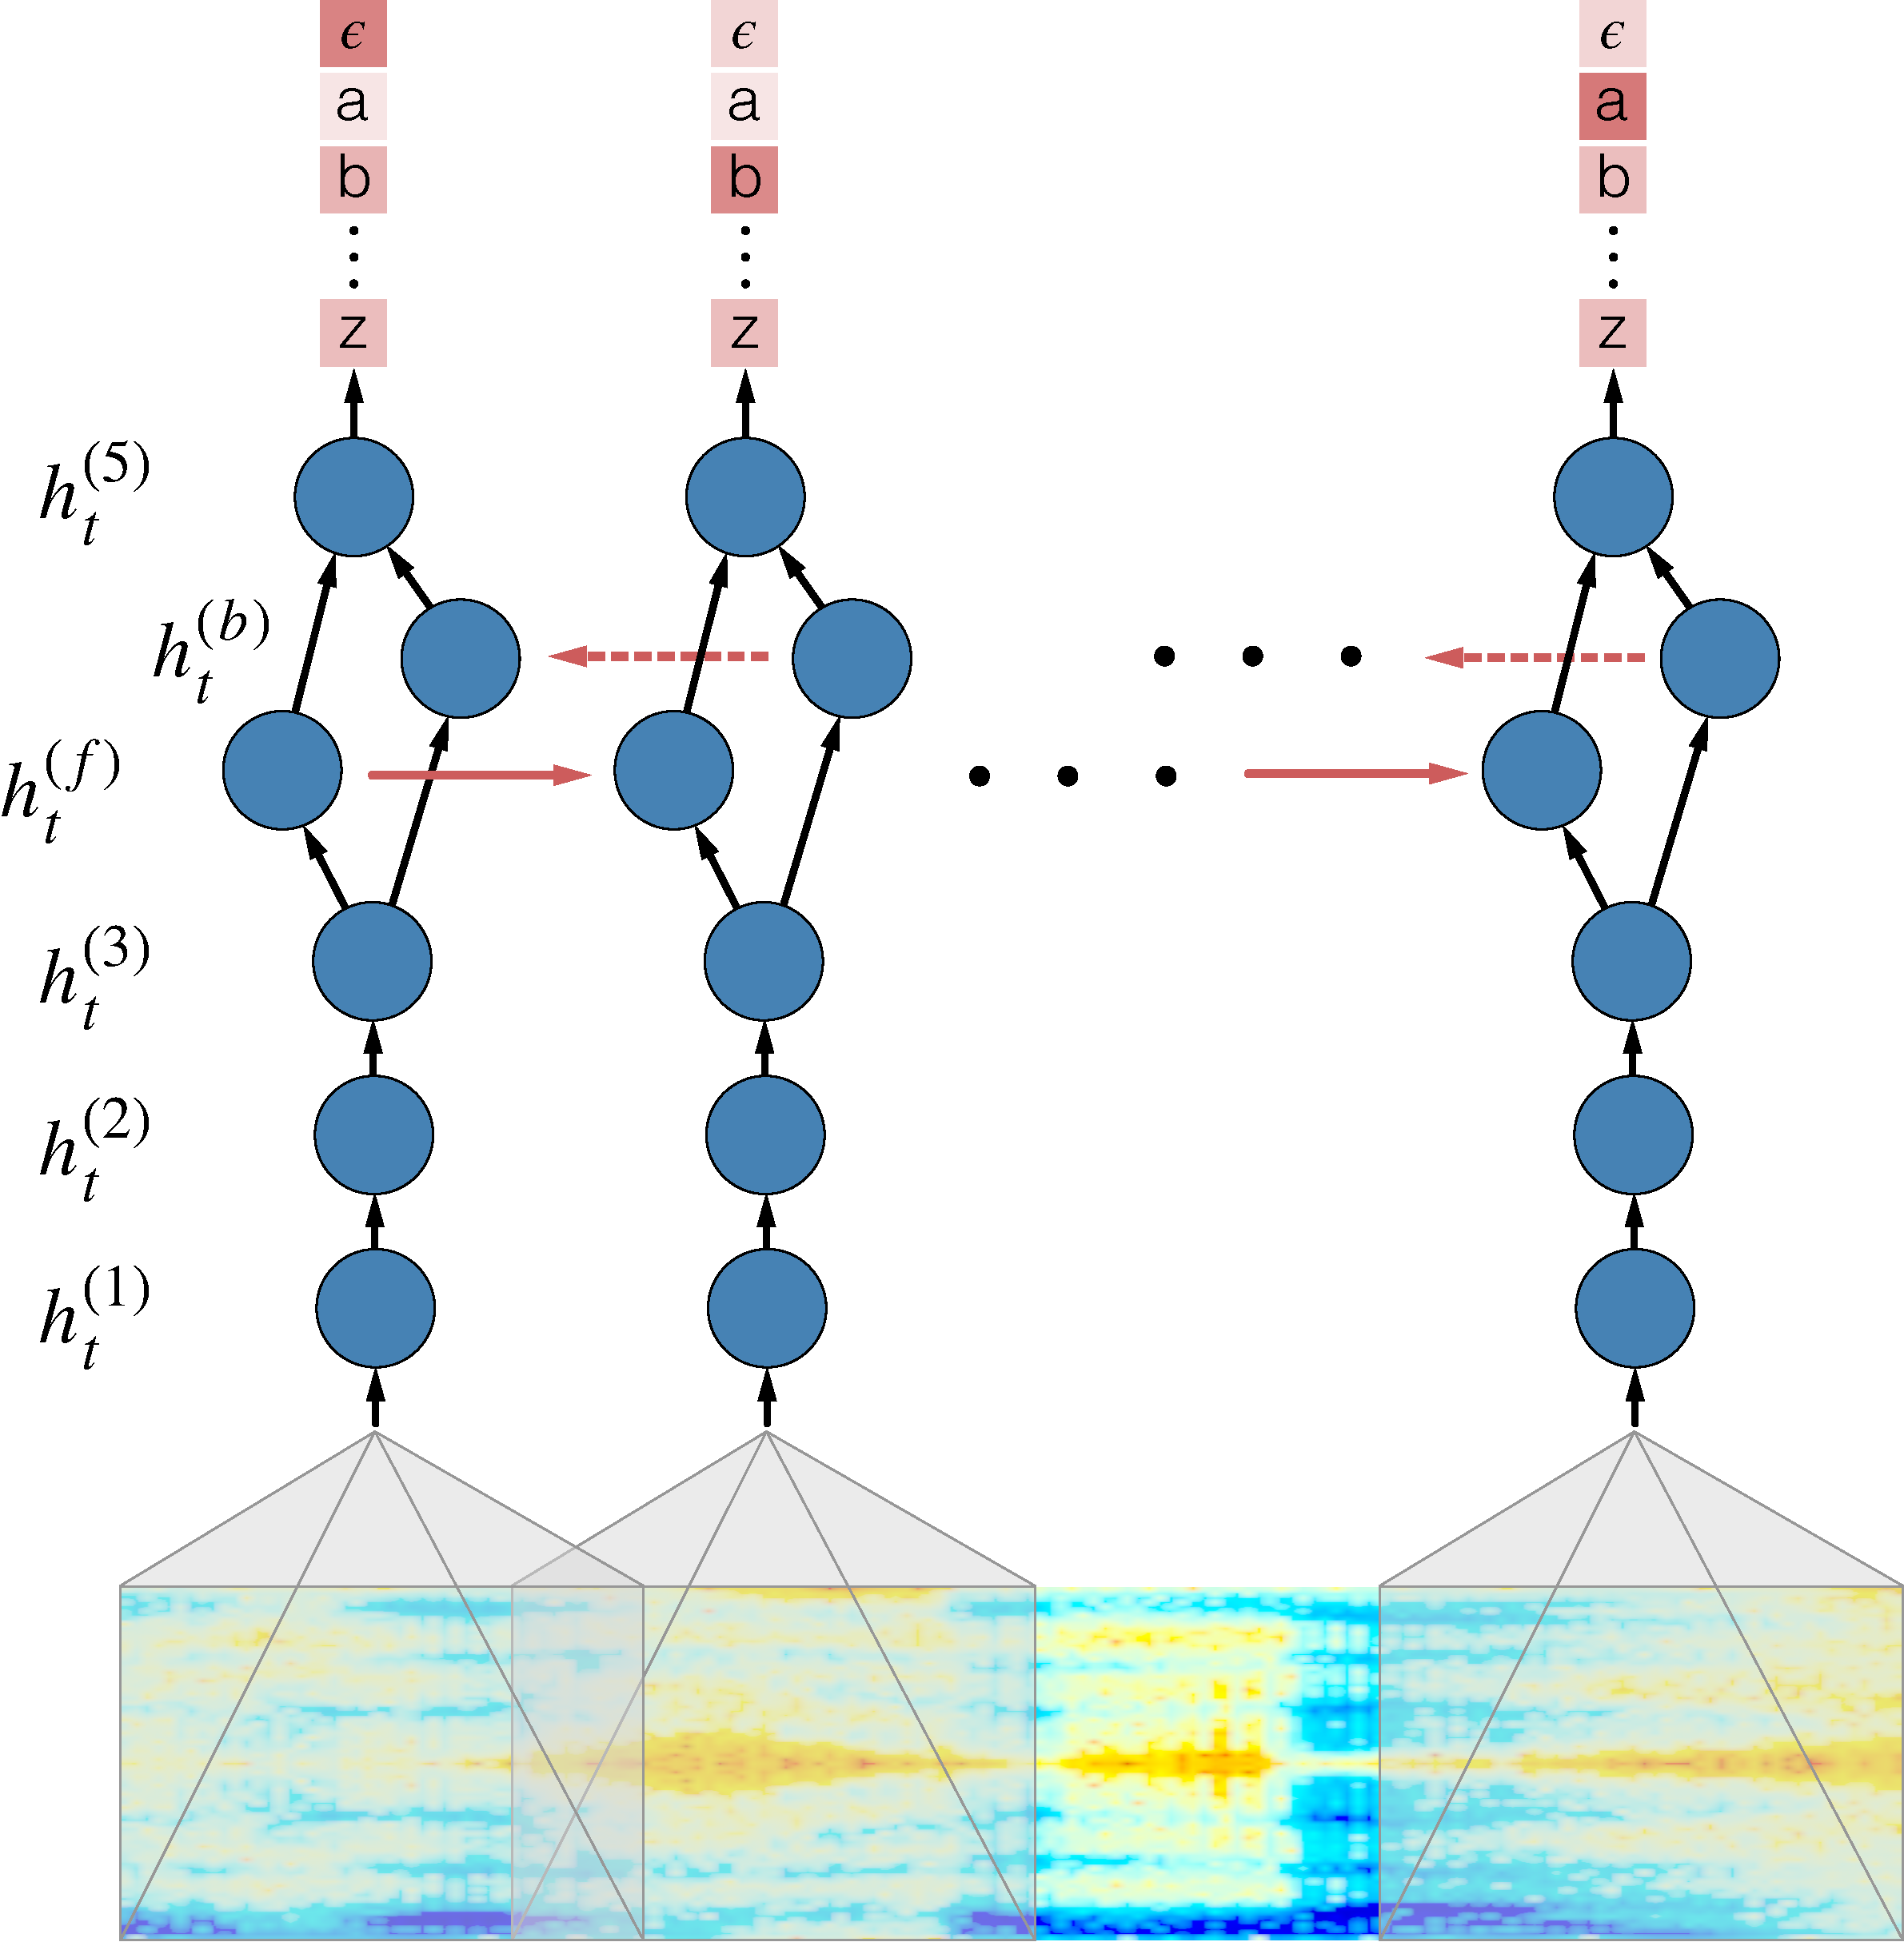
\includegraphics[width=0.6\textwidth]{deepspeech/figures/speech_network.pdf}
  \caption{Structure of our RNN model and notation.}
  \label{fig:deepspeech:rnn}
\end{figure}

The complete RNN model is illustrated in Figure~\ref{fig:deepspeech:rnn}. Note
that its structure is considerably simpler than related models from the
literature~\cite{graves2014}---we have limited ourselves to a single recurrent
layer (which is the hardest to parallelize) and we do not use
Long-Short-Term-Memory (LSTM) circuits. One disadvantage of LSTM cells is that
they require computing and storing multiple gating neuron responses at each
step. Since the forward and backward recurrences are sequential, this small
additional cost can become a computational bottleneck. By using a homogeneous
model we have made the computation of the recurrent activations as efficient as
possible: computing the ReLu outputs involves only a few highly optimized BLAS
operations on the GPU and a single point-wise nonlinearity.

\subsection{Regularization}

While we have gone to significant lengths to expand our datasets (c.f.
Section~\ref{sec:deepspeech:data}), the recurrent networks we use are still
adept at fitting the training data. In order to reduce variance further, we use
several techniques.  

During training we apply a dropout~\cite{hinton2012dropout} rate between 5\% -
10\%. We apply dropout in the feed-forward layers but not to the recurrent
hidden activations.

A commonly employed technique in computer vision during network evaluation is
to randomly jitter inputs by translations or reflections, feed each jittered
version through the network, and vote or average the
results~\cite{krizhevsky2012imagenet}. Such jittering is not common in ASR,
however we found it beneficial to translate the raw audio files by 5ms (half
the filter bank step size) to the left and right, then forward propagate the
recomputed features and average the output probabilities. At test time we also
use an ensemble of several RNNs, averaging their outputs in the same way.

\subsection{Language Model}
\label{sec:deepspeech:languagemodel}

When trained from large quantities of labeled speech data, the RNN model can
learn to produce readable character-level transcriptions. Indeed for many of
the transcriptions, the most likely character sequence predicted by the RNN is
exactly correct without external language constraints. The errors made by the
RNN in this case tend to be phonetically plausible renderings of English
words---Table~\ref{table:deepspeech:max_decoded} shows some examples. Many of
the errors occur on words that rarely or never appear in our training set. In
practice, this is hard to avoid:  training from enough speech data to
\emph{hear} all of the words or language constructions we might need to know is
impractical.  Therefore, we integrate our system with an N-gram language model
since these models are easily trained from huge unlabeled text corpora. For
comparison, while our speech datasets typically include up to 3 million
utterances, the N-gram language model used for the experiments in
Section~\ref{sec:deepspeech:expnoise} is trained from a corpus of 220 million
phrases, supporting a vocabulary of 495,000 words.\footnote{We use the KenLM
toolkit~\cite{heafield2013} to train the N-gram language models in our
experiments.} 

\begin{table}[h]
\centering
\begin{tabular}{l | l}
\toprule
RNN output  & Decoded Transcription \\
\midrule
\rule{0pt}{2ex}
what is the weather like in & what is the weather like in \\
\rule{0pt}{0.1ex}
bostin right now       & boston right now \\
\rule{0pt}{4ex}
prime miniter nerenr modi   & prime minister narendra modi \\ 
\rule{0pt}{4ex}
arther n tickets for the game  & are there any tickets for the game \\ 
\bottomrule
\end{tabular}
\caption{Examples of transcriptions directly from the RNN (left) with errors
         that are fixed by addition of a language model (right).}
\label{table:deepspeech:max_decoded}
\end{table}

We perform a search to find the sequence of characters that is most probable
according to both the RNN output and the language model (where the language
model interprets the string of characters as words). Specifically, we aim to
find a sequence $Y$ that maximizes the combined objective:
\begin{align*}
    Q(Y) = \log(p(Y \mid X)) + \alpha \log(p_{\text{lm}}(Y)) + \beta \textrm{ word\_count}(Y)
\end{align*}
where $\alpha$ and $\beta$ are tunable parameters (set by cross-validation)
that control the trade-off between the RNN, the language model constraint and
the length of the sentence. The term $p_{\text{lm}}$ denotes the
probability of the sequence $c$ according to the N-gram model. We maximize
this objective using a highly optimized beam search algorithm, with a typical
beam size in the range 1000-8000---similar to the approach described by Hannun
et al.~\cite{hannun2014firstpass}.

%
%\begin{figure}
%  \centering
%  \includegraphics[width=\linewidth]{figs/results}
%  \caption{
%    Evaluated on the test set, the model outperforms the average cardiologist score on both the Sequence and the Set F1 metrics.
%  }
%  \label{fig:model_vs_cardiol}
%\end{figure}
%
%\section{Data}
%\label{data}
%\section{Training Data}
\label{sec:deepspeech:data}

Large-scale deep learning systems require an abundance of labeled data. For our
system we need many recorded utterances and corresponding English
transcriptions, but there are few public datasets of sufficient scale. To train
our largest models we have thus collected an extensive dataset consisting of
5000 hours of read speech from 9600 speakers. For comparison, we have
summarized the labeled datasets available to us in
Table~\ref{table:deepspeech:datasets}.

\begin{table}[]
\centering
\begin{tabular}{l c c c}
 \toprule
 Dataset & Type & Hours & Speakers  \\
 \midrule
 WSJ         & read           &   80 & 280 \\
 Switchboard & conversational &  300 & 4000 \\
 Fisher      & conversational & 2000 & 23000 \\
 Baidu       & read           & 5000 & 9600 \\
 \bottomrule
\end{tabular}
\caption{A summary of the datasets used to train Deep Speech. The Wall Street
         Journal, Switchboard and Fisher~\cite{cieri2004fisher} corpora are all
         published by the Linguistic Data Consortium.}
\label{table:deepspeech:datasets}
\end{table}

\subsection{Synthesis by superposition}
\label{sec:deepspeech:noisesynth}

To expand our potential training data even further we use data synthesis, which
has been successfully applied in other contexts to amplify the effective number
of training samples~\cite{sapp2008, lecun2004, coates2011}. In our work, the
goal is primarily to improve performance in noisy environments where existing
systems break down. Capturing labeled data (e.g., read speech) from noisy
environments is not practical, however, and thus we must find other ways to
generate such data.

To a first order, audio signals are generated through a process of
superposition of source signals. We can use this fact to synthesize noisy
training data. For example, if we have a speech audio track $x^{(i)}$ and a
``noise'' audio track $\xi^{(i)}$, then we can form the ``noisy speech'' track
$\hat{x}^{(i)} = x^{(i)}+\xi^{(i)}$ to simulate audio captured in a noisy
environment. If necessary, we can add reverberations, echoes or other forms of
damping to the power spectrum of $\xi^{(i)}$ or $x^{(i)}$ and then simply add
them together to make fairly realistic audio scenes.

There are, however, some risks in this approach. For example, in order to take
1000 hours of clean speech and create 1000 hours of noisy speech, we will need
unique noise tracks spanning roughly 1000 hours. We cannot settle for, say, 10
hours of repeating noise, since it may become possible for the recurrent
network to memorize the noise track and ``subtract'' it out of the synthesized
data. Thus, instead of using a single noise source $\xi^{(i)}$ with a length of
1000 hours, we use a large number of shorter clips (which are easier to collect
from public video sources) and treat them as separate sources of noise before
superimposing all of them: $\hat{x}^{(i)} = x^{(i)} + \xi_1^{(i)} +\xi_2^{(i)}
+ \ldots$.

When superimposing many signals collected from video clips, we can end up with
``noise'' sounds that are different from the kinds of noise recorded in real
environments. To ensure a good match between our synthetic data and real data,
we rejected any candidate noise clips where the average power in each frequency
band differed significantly from the average power observed in real noisy
recordings.

\subsection{Capturing Lombard Effect}
\label{sec:deepspeech:lombard}

One challenging effect encountered by speech recognition systems in noisy
environments is the ``Lombard Effect''~\cite{junqua1993lombard}: speakers
actively change the pitch or inflections of their voice to overcome noise
around them. This (involuntary) effect does not show up in recorded speech
datasets since they are collected in quiet environments. To ensure that the
effect is represented in our training data we induce the Lombard effect
intentionally during data collection by playing loud background noise through
headphones worn by a person as they record an utterance. The noise induces them
to inflect their voice, thus allowing us to capture the Lombard effect in our
training data.\footnote{We have experimented with noise played through
headphones as well as through computer speakers. Using headphones has the
advantage that we obtain ``clean'' recordings without the background noise
included and can add our own synthetic noise afterward.}


%
%\input{comparison}
%\section{Results}
%\label{results}
%\section{Experimental Results}

\subsection*{Evaluation Metrics}
We use two metrics to measure model accuracy, using the cardiologist committee
annotations as the ground truth.

\textbf{Sequence Level Accuracy (F1):} We measure the average overlap between
the prediction and the ground truth sequence labels. For every record, a model
is required to make a prediction approximately once per second (every 256
samples). These predictions are compared against the ground truth annotation.

\textbf{Set Level Accuracy (F1):} Instead of treating the labels for a record
as a sequence, we consider the set of unique arrhythmias present in each 30
second record as the ground truth annotation. Set Level Accuracy, unlike
Sequence Level Accuracy, does not penalize for time-misalignment within a
record. We report the F1 score between the unique class labels from the ground
truth and those from the model prediction.

In both the Sequence and the Set case, we compute the metrics for each class
separately. We then compute aggregate results for AUC and F1 as the
class-frequency weighted mean.

\subsection*{Model and Cardiologist Performance}

We assess the cardiologist performance on the test set. Recall that each of the
records in the test set has a ground truth label from a committee of three
cardiologists as well as individual labels from a disjoint set of 6 other
cardiologists. To assess cardiologist performance for each class, we take the
average of all the individual cardiologist scores using the group label as the
ground truth annotation.

\begin{table}
\centering
\begin{small}
\begin{tabular}{r l l}
\toprule
                               & Sequence AUC & Set AUC \\
\midrule
Atrial Fibrillation \& Flutter & 0.975 & 0.959 \\
Atrio-ventricular Block        & 0.989 & 0.981 \\
Bigeminy                       & 0.998 & 0.997 \\
Ectopic Atrial Rhythm          & 0.908 & 0.935 \\
Idioventricular Rhythm         & 0.995 & 0.986 \\
Junctional Rhythm              & 0.985 & 0.980 \\
Noise                          & 0.985 & 0.958 \\
Sinus Rhythm                   & 0.976 & 0.981 \\
Supraventricular Tachycardia   & 0.972 & 0.940 \\
Trigeminy                      & 0.999 & 0.997 \\
Ventricular Tachycardia        & 0.995 & 0.981 \\
Wenckebach                     & 0.982 & 0.981 \\
\midrule
   Average                     & 0.979               & 0.974 \\
\bottomrule
\end{tabular}
\end{small}
\caption{The model AUC scores for each rhythm class and in aggregate.}
\label{tab:arrhythmias:model_auc}
\end{table}

Table~\ref{tab:arrhythmias:model_auc} gives the per class and aggregate AUC
scores. Our model achieves an AUC of greater than 0.90 for each of the 12
rhythm diagnoses, with an average AUC of 0.97. We also compute the sensitivity
at a specifity of 0.9 and vice versa in~\ref{tab:arrhythmias:sens_spec}.

\begin{table}
\centering
\begin{small}
\begin{tabular}{r l l}
\toprule
             & Sensitivity       & Specificity  \\
\midrule
Atrial Fibrillation \& Flutter & 0.923 & 0.914 \\
Atrio-ventricular Block        & 0.991 & 0.964 \\
Bigeminy                       & 1.000 & 0.997 \\
Ectopic Atrial Rhythm          & 0.754 & 0.665 \\
Idioventricular Rhythm         & 0.990 & 0.990 \\
Junctional Rhythm              & 0.982 & 0.959 \\
Noise                          & 0.965 & 0.968 \\
Sinus Rhythm                   & 0.934 & 0.946 \\
Supraventricular Tachycardia   & 0.958 & 0.925 \\
Trigeminy                      & 1.000 & 0.999 \\
Ventricular Tachycardia        & 1.000 & 0.981 \\
Wenckebach                     & 0.977 & 0.956 \\
\bottomrule
\end{tabular}
\end{small}
\caption{The maximum model sensitivity with specificity greater than 0.9 and
         vice versa.}
\label{tab:arrhythmias:sens_spec}
\end{table}

\begin{table}
\centering
\begin{small}
\begin{tabular}{r c c c c}
\toprule
    & \multicolumn{2}{c}{Sequence F1} & \multicolumn{2}{c}{Set F1} \\
\cmidrule{2-5}
 & Model & Cardiol. & Model & Cardiol. \\
\midrule
Atrial Fibrillation \& Flutter & 0.802 & 0.679 & 0.817 & 0.687 \\
Atrio-ventricular Block        & 0.850 & 0.769 & 0.830 & 0.756 \\
Bigeminy                       & 0.896 & 0.837 & 0.870 & 0.849 \\
Ectopic Atrial Rhythm          & 0.537 & 0.476 & 0.545 & 0.529 \\
Idioventricular Rhythm         & 0.751 & 0.632 & 0.818 & 0.720 \\
Junctional Rhythm              & 0.640 & 0.684 & 0.778 & 0.674 \\
Noise                          & 0.852 & 0.768 & 0.704 & 0.689 \\
Sinus Rhythm                   & 0.886 & 0.847 & 0.934 & 0.907 \\
Supraventricular Tachycardia   & 0.458 & 0.449 & 0.630 & 0.556 \\
Trigeminy                      & 0.909 & 0.843 & 0.870 & 0.816 \\
Ventricular Tachycardia        & 0.520 & 0.566 & 0.653 & 0.769 \\
Wenckebach                     & 0.714 & 0.593 & 0.806 & 0.736 \\
\midrule
Average	                       & 0.808 & 0.750 & 0.809 & 0.778 \\
\bottomrule
\end{tabular}
\end{small}
\caption{The F1 score for the sequence and set-level metrics comparing the
         model and the average of six individual cardiologist to the committee
         consensus ground truth.}
\label{tab:arrhythmias:model_cardiologist_f1}
\end{table}

Table~\ref{tab:arrhythmias:model_cardiologist_f1} shows the breakdown of both
cardiologist and model sequence and set F1 across the different rhythm classes.
The model outperforms the average cardiologist performance on most rhythms,
noticeably outperforming the cardiologists in the AV Block set of arrhythmias
which includes Mobitz I (Wenckebach), Mobitz II and complete heart block (both
categorized as Atrio-ventricular Block). This is especially useful given the
severity of second and third degree heart block and the importance of
distinguishing these two from Wenckebach which is usually considered benign.
The model also outperforms the cardiologist average accross all rhythm classes
for both the sequence and set F1 score.

\begin{figure}
\centering
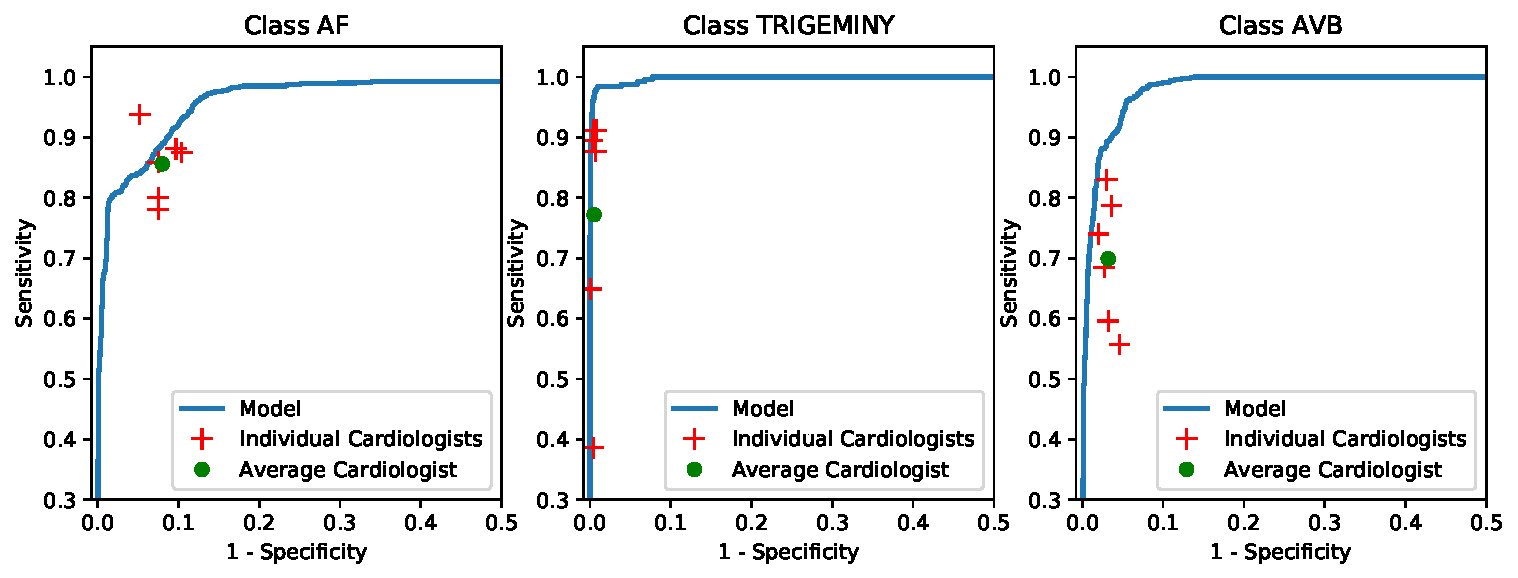
\includegraphics[width=1.0\textwidth]{arrhythmias/figures/roc_curve.pdf}
\caption{Receiver operating characteristic curves at the sequence level for
    atrial fibrillation and flutter (AF), trigeminy and atrioventricular block
    (AVB).}
\label{fig:arrhythmias:roc_curve}
\end{figure}

Figures~\ref{fig:arrhythmias:roc_curve} and
\ref{fig:arrhythmias:prec_recall_curve} show the models performance at various
operating thresholds on an ROC and precision-recall curve respectively. We show
here three arrhythmias taken from one-third of the test set. We also compute
and plot the operating point for the six individual cardiologists who annotated
that third of the test set. The model outperforms almost all of the individual
cardiologists. We see the same behaviour for the other rhythm classes not shown
here.

\begin{figure}
\centering
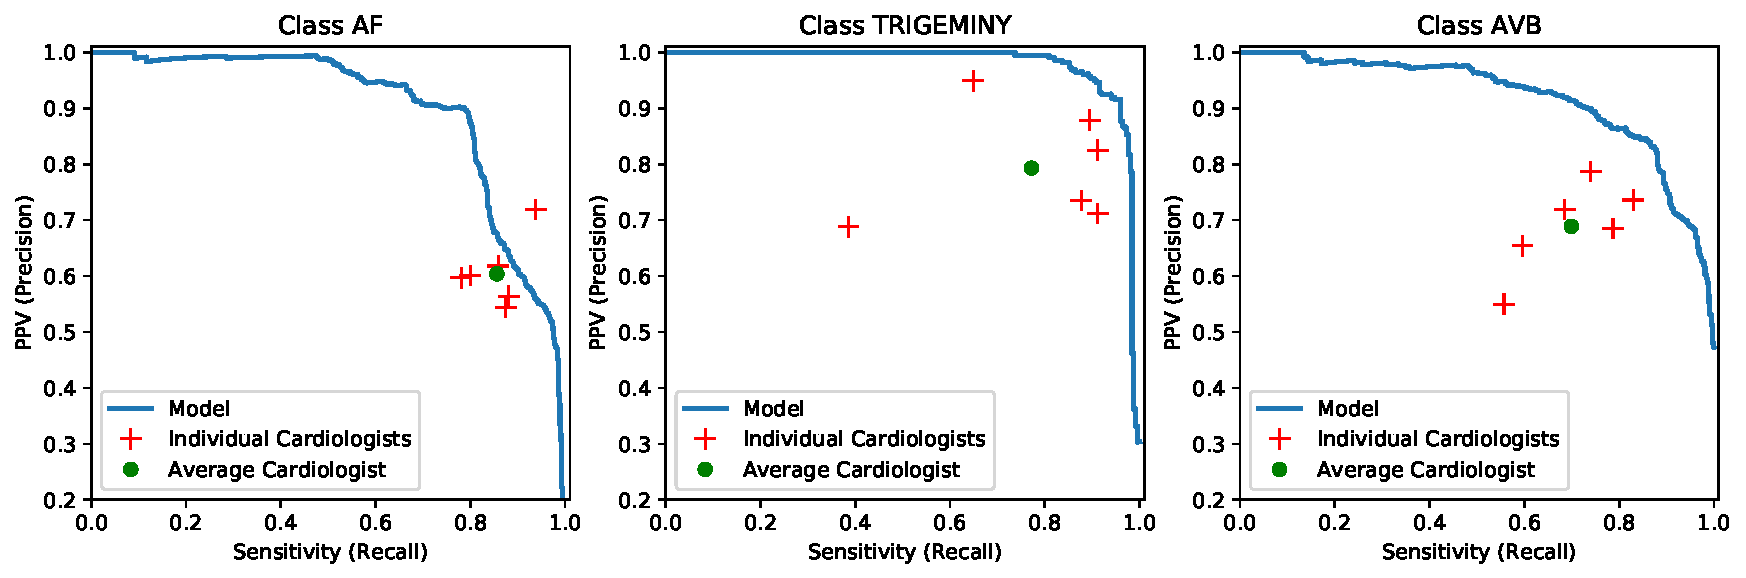
\includegraphics[width=1.0\textwidth]{arrhythmias/figures/prec_recall_curve.pdf}
    \caption{Precision-recall curves at the sequence level for atrial
    fibrillation and flutter (AF), trigeminy and atrioventricular block (AVB).}
\label{fig:arrhythmias:prec_recall_curve}
\end{figure}

%
%\section{Analysis}
%\label{analysis}
%\section{Analsysis}

The model outperforms the average cardiologist score on both the sequence and
the set F1 metrics. Figure~\ref{fig:confusion} shows a confusion matrix of the
model predictions on the test set. Many arrhythmias are confused with the sinus
rhythm. We expect that part of this is due to the sometimes ambiguous location
of the exact onset and offset of the arrhythmia in the ECG record.

\begin{figure}
\begin{subfigure}{.5\textwidth}
  \centering
  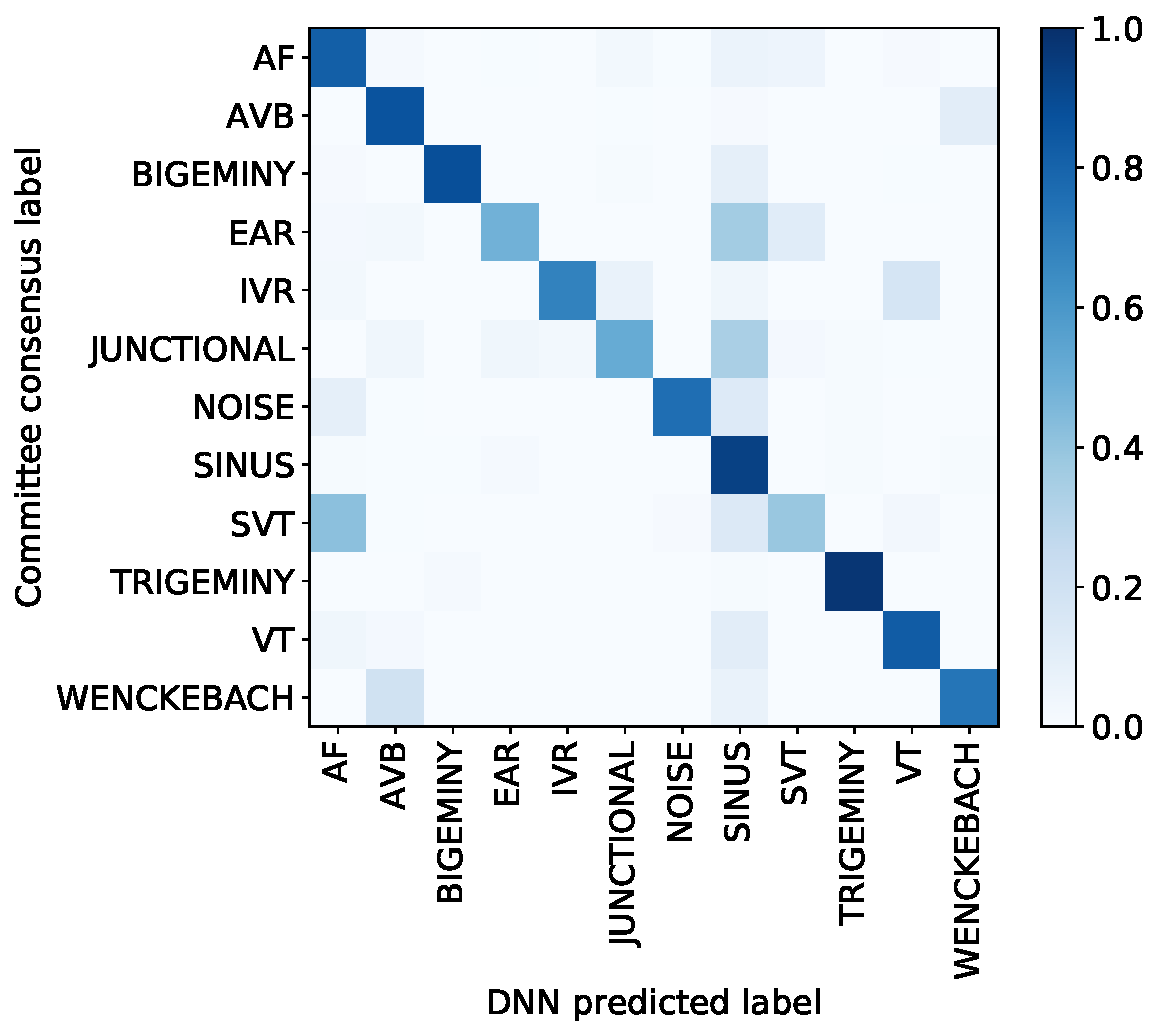
\includegraphics[width=0.9\linewidth]{arrhythmias/figures/model_confusions.pdf}
  \caption{Model}
  \label{fig:arrhythmia:model_confusion}
\end{subfigure}
\begin{subfigure}{.5\textwidth}
  \centering
  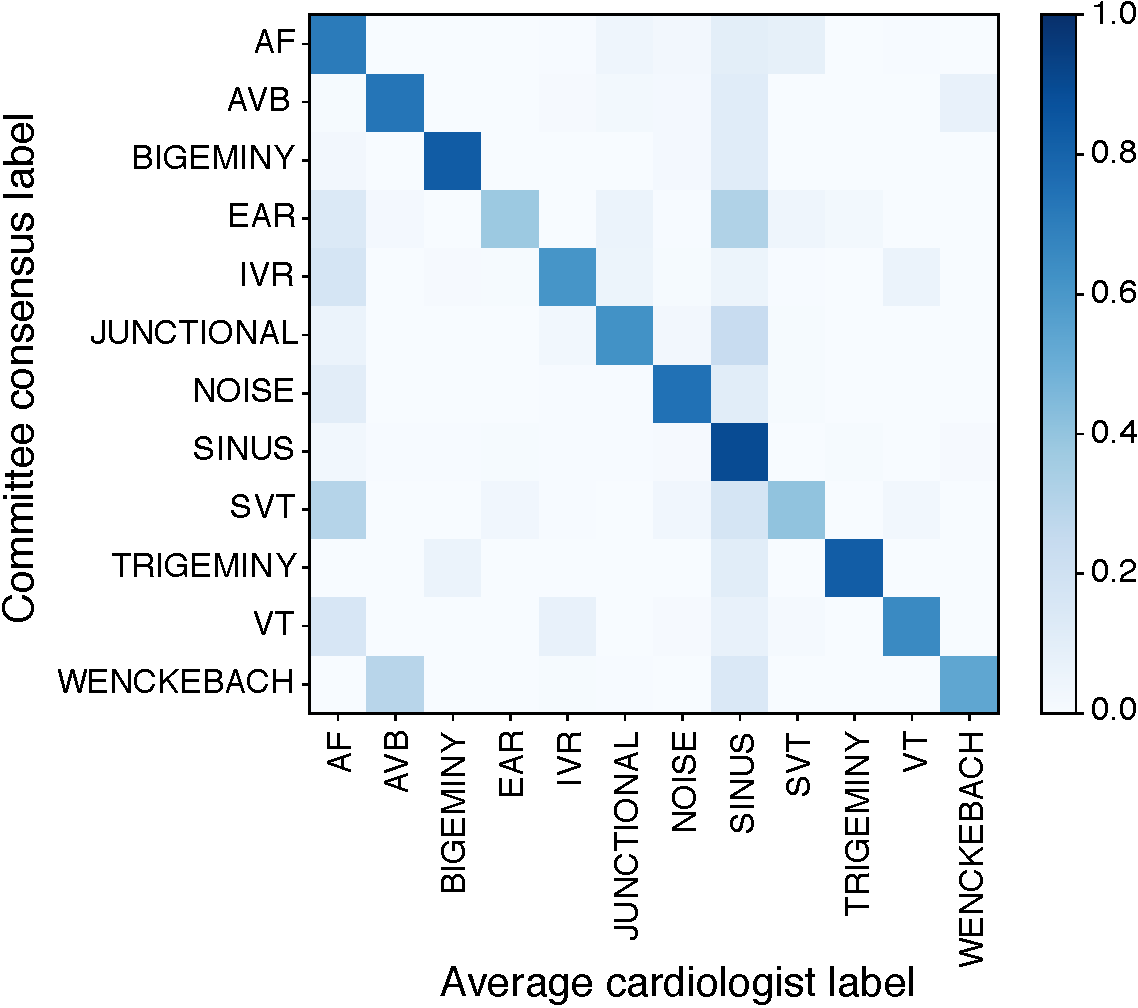
\includegraphics[width=0.9\linewidth]{arrhythmias/figures/human_confusions.pdf}
  \caption{Individual Cardiologists}
  \label{fig:arrhythmia:human_confusion}
\end{subfigure}
\caption{Confusion matrices for the model and individual cardiologist
         predictions with the committee consensus annotations as ground
         truth.}
\end{figure}

Often the mistakes made by the model are understandable. For example, confusing
Wenckebach and AVB\_Type2 makes sense given that the two rhythms in general
have very similar ECG morphologies. Similarly, Supraventricular Tachycardia
(SVT) and Atrial Fibrillation (AFIB) are often confused with Atrial Flutter
(AFL) which is understandable given that they are all atrial arrhythmias. We
also note that Idioventricular Rhythm (IVR) is sometimes mistaken as
Ventricular Tachycardia (VT), which again makes sense given that the two only
differ in heart-rate and are difficult to distinguish close to the 100 beats
per minute delineation.

One of the most common confusions is between Ectopic Atrial Rhythm (EAR) and
the sinus rhythm. The main distinguishing criteria for this rhythm is an
irregular P wave. This can be subtle to detect especially when the P wave has a
small amplitude or when noise is present in the signal.


%\begin{figure}[t]
%  \centering
%  \includegraphics[width=\linewidth]{figs/confusion.pdf}
%  \caption{
%    A confusion matrix for the model predictions on the test set. Many of the mistakes the model makes are not surprising. For example, confusing second degree AV Block (Type 2) with Wenckebach makes sense given the often similar expression of the two arrhythmias in the ECG record.
%  }
%  \label{fig:confusion}
%\end{figure}
%\section{Related Work}
%\label{related}
%\section{Related Work}
\label{sec:deepspeech:related}

Several parts of our work are inspired by previous results. Neural network
acoustic models and other connectionist approaches were first introduced to
speech pipelines in the early 1990s~\cite{bourlard93, renals1994, ellis1999}.
These systems, similar to DNN acoustic models~\cite{mohamed2011, hinton2012,
dahl2011a}, replace only one stage of the speech recognition pipeline.
Mechanically, our system is similar to other efforts to build end-to-end speech
systems from deep learning algorithms. For example,
Graves~et~al.~\cite{graves2006} have previously introduced the ``Connectionist
Temporal Classification'' (CTC) loss function for scoring transcriptions
produced by RNNs and, with LSTM networks, have previously applied this approach
to speech~\cite{graves2014}. We similarly adopt the CTC loss for part of our
training procedure but use much simpler recurrent networks with
rectified-linear activations~\cite{glorot2011, maas2013, nair2010}. Our
recurrent network is similar to the bidirectional RNN used by Hannun et
al.~\cite{hannun2014firstpass}, but with multiple changes to enhance its
scalability. By focusing on scalability, we have shown that these simpler
networks can be effective even without the more complex LSTM machinery.

Our work is certainly not the first to exploit scalability to improve
performance of DL algorithms. The value of scalability in deep learning is
well-studied~\cite{coates2011b, le2013} and the use of parallel processors
(including GPUs) has been instrumental to recent large-scale DL
results~\cite{szegedy2015, le2013}. Early ports of DL algorithms to GPUs
revealed significant speed gains~\cite{raina2009}. Researchers have also begun
choosing designs that map well to GPU hardware to gain even more efficiency,
including convolutional~\cite{krizhevsky2012imagenet, ciresan2011,
sainath2013b} and locally connected~\cite{coates2013cotshpc, ciresan2012}
networks, especially when optimized libraries like
cuDNN~\cite{chetlur2014cudnn} and BLAS are available. Indeed, using
high-performance computing infrastructure, it is possible today to train neural
networks with more than 10 billion connections~\cite{coates2013cotshpc} using
clusters of GPUs. These results inspired us to focus first on making scalable
design choices to efficiently utilize many GPUs before trying to engineer the
algorithms and models themselves.

With the potential to train large models, there is a need for large training
sets as well. In other fields, such as computer vision, large labeled training
sets have enabled significant leaps in performance as they are used to feed
larger and larger DL systems~\cite{szegedy2015, krizhevsky2012imagenet}. In
speech recognition, however, such large training sets are less common, with
typical benchmarks having training sets ranging from tens of hours (e.g. the
Wall Street Journal corpus with 80 hours) to several hundreds of hours (e.g.
Switchboard and Broadcast News). Larger benchmark datasets, such as the Fisher
corpus~\cite{cieri2004fisher} with 2000 hours of transcribed speech, are rare
and only recently being studied. To fully utilize the expressive power of the
recurrent networks available to us, we rely not only on large sets of labeled
utterances, but also on synthesis techniques to generate novel examples. This
approach is well known in computer vision~\cite{sapp2008, lecun2004,
coates2011} but we have found this especially convenient and effective for
speech when done properly.


%\section{Conclusion}
%\label{conclusion}

%\section{Conclusion}

We presented a decoding algorithm which enables first-pass LVCSR with a
language model for CTC-trained neural networks. This decoding approach removes
the lingering dependence on HMM-based systems found in previous work.
Furthermore, first-pass decoding demonstrates the capabilities of a CTC-trained
system without the confounding factor of potential effects from pruning the
search space via a provided lattice. While our results do not outperform the
best HMM-based systems on the WSJ corpus, they demonstrate the promise of
CTC-based speech recognition systems.

Our experiments with the BRNN further simplify the infrastructure needed to
create CTC-based speech recognition systems. The BRNN is overall a less complex
architecture than LSTMs and can relatively easily be made to run on GPUs since
large matrix multiplications dominate the computation. However, our experiments
suggest that recurrent connections are critical for good performance.
Bi-directional recurrence helps beyond unidirectional recurrence but could be
sacrificed in cases that require low-latency, online speech recognition. Taken
together with previous work on CTC-based LVCSR, we believe there is an exciting
path forward for high quality LVCSR without the complexity of HMM-based
infrastructure.

%\input{rhythms}
